\chapter{Mathematical Model of Type-3 Wind Turbine Generators}

\label{ch: Mod}

TOPSTER

\section{Mathematical Model 1}

Proposed by \cite{Erlich2012}, this mathematical model is able to represent the dynamic of both Type-3 and -4 WTG's and can be used to simulate entire wind power plants. In this model, a Thevenin equivalent circuit is connected to grid with a controlled voltage source, as depicted in Figure \ref{fig: ErlMod}. 

\begin{figure}[h]
	\caption{Type-3 WTG model proposed by Erlich}
	\begin{center}
		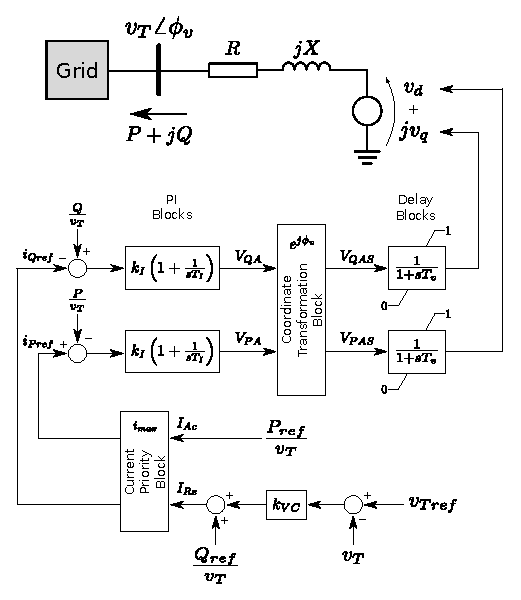
\includegraphics[scale=1]{Images/ErlichModel.eps}
	\end{center}
	\label{fig: ErlMod}
	\legend{Source: Adapted from \cite{Erlich2012}}
\end{figure}

Terminal voltage $v_{T}$ is the variable of interest in this model, appearing as input to DFIG's control system. Active and reactive current are calculated using that input, according to equation \eqref{eq: Currents}.

\begin{equation}
	\begin{cases}
		I_{Ac} = \frac{v_{T}}{p_{Tref}} \\
		I_{Re} = k_{VC}(v_{Tref} - v_{T})
	\end{cases}
	\label{eq: Currents}
\end{equation}

The calculated currents feed a current priority block. This block analyses the current magnitude and terminal voltage level and decides whether power injection or voltage control will be prioritize. In summary, it checks if the generator's current is below a maximum level $i_{max}$ and, if it is not, the block verifies if terminal voltage is above a threshold value $v^{*}$ to decide what will be prioritized. The following algorithm describes the current priority block operation.

\begin{center}
	\begin{lstlisting}[mathescape, columns=fullflexible]
	if $\sqrt{I_{Ac}^{2} + I_{Re}^{2}} \leq i_{max}$ then:
		$\begin{cases}
				i_{Pref} = I_{Ac} \\
				i_{Qref} = I_{Re}
		\end{cases}$
	else:
		if $v_{T} \geq v^{*}$ then:	
			$\begin{cases}
				i_{Pref} = min(i_{max}, I_{Ac}) \\
				i_{Qref} = \sqrt{i_{max}^{2} - i_{Pref}^{2}}
			\end{cases}$
		else:
			$\begin{cases}
				i_{Qref} = min(i_{max}, I_{Re}) \\
				i_{Pref} = \sqrt{i_{max}^{2} - i_{Qref}^{2}}
			\end{cases}$
	\end{lstlisting}
\end{center}

The following PI blocks stand for the DFIG controllers (blade, gearbox, rotor-side and grid-side converters controllers) and their outputs follow the equations presented in \eqref{eq: PI}.

\begin{equation}
	\begin{cases}
		V_{PA} = k_{I}[(i_{Pref} - \frac{p}{v_{T}}) +\frac{1}{T_{I}}\int\displaylimits_{0}^{t}	(i_{Pref} - \frac{p}{v_{T}})dt]\\
		\\
		V_{QA} = k_{I}[(\frac{q}{v_{T}} - i_{Qref}) +\frac{1}{T_{I}}\int\displaylimits_{0}^{t}	(\frac{q}{v_{T}} - i_{Qref})dt]
	\end{cases}
	\label{eq: PI}
\end{equation}

Until here the controller operates on terminal voltage oriented coordinates, so a coordinate transformation block is needed to adequate to synchronous grid coordinates. This block operates according to equations \eqref{eq: CoordShift}.

\begin{equation}
	\begin{cases}
		V_{PAS} = -V_{PA}cos(\theta_{v}) - V_{QA}sin(\theta_{v}) \\
		V_{QAS} = V_{PA}sin(\theta_{v}) - V_{QA}cos(\theta_{v})
	\end{cases}
	\label{eq: CoordShift}
\end{equation}

Last, two delay blocks supplying the voltage source (one for each component $d$ and $q$) simulate the delay effects of the electrical machine and the back-to-back converter. Their effects are described by \eqref{eq: DelayBlocks}.

\begin{equation}
	\begin{cases}
		\dot{v}_{d} = \frac{1}{T_{V}}(v_{d} - V_{PAS}) \\
		\dot{v}_{q} = \frac{1}{T_{V}}(v_{q} - V_{QAS})
	\end{cases}
	\label{eq: DelayBlocks}
\end{equation}

The outputs of this model are real and reactive power produced (or consumed) by the WTG and their equations are shown below.

\begin{equation}
	\begin{cases}
		P_{e} = \frac{r(v_{Td}v_{d} + v_{Tq}v_{q} - v_{T}^{2}) + x(v_{Tq}v_{d} - v_{Td}v_{q})}{r^{2} + x^{2}} \\
		Q_{e} = \frac{x(v_{Td}v_{d} + v_{Tq}v_{q} - v_{T}^{2}) - r(v_{Tq}v_{d} - v_{Td}v_{q})}{r^{2} + x^{2}}
	\end{cases}
	\label{eq: Outputs}
\end{equation}

Thus, this model can be interpreted as follows:

\begin{equation}
	\begin{cases}
		\dot{x} = f(x, u, y, p) \\
		y = g(x, u, y, p)
	\end{cases}
	\label{eq: xdot}
\end{equation}

\noindent where the state variables $x$, inputs $u$, outputs $y$ and parameters $p$ vectors are described by \eqref{eq: x}, \eqref{eq: u}, \eqref{eq: y} and \eqref{eq: p}, respectively.

\begin{equation}
	x = [v_{d}, v_{q}]^T
	\label{eq: x}
\end{equation}

\begin{equation}
	u = [v_{T}, \theta_{v}, P, Q]^T
	\label{eq: u}
\end{equation}

\begin{equation}
	y = [P_{e}, Q_{e}]^T
	\label{eq: y}
\end{equation}

\begin{equation}
	p = [r, x, k_{I}, T_{I}, T_{V}, k_{VC}]^T
	\label{eq: p}
\end{equation}

In \eqref{eq: p}, the parameters correspond to the stator equivalent resistance $r$ and reactance $x$, PI gain $k_{I}$ and time constant $T_{I}$, delay block time constant $T_{V}$ and voltage block gain $k_{VC}$.